\documentclass[notheorems]{beamer}

%packages
\usepackage[utf8]{inputenc}
\usepackage[english]{babel}
\usepackage{float}
\usepackage{tikz}
\usepackage{pgfplots}
\usepackage{geometry}
\usepackage{amsfonts, amssymb, amsmath}             % Fonte e símbolos matemáticos
%\usepackage[english,ruled,lined,linesnumbered]{algorithm2e}    % Escrever algoritmos
\usepackage{algorithm,algorithmic}
\usepackage{amsthm}
\usepackage{theoremref}
\usepackage[autostyle]{csquotes}
\usepackage{multicol}
\usepackage{biblatex}
%biber latex settings
\addbibresource{mybib.bib}

\usepackage[utf8]{inputenc}

\addtobeamertemplate{navigation symbols}{}{%
  \usebeamerfont{footline}%
  \usebeamercolor[fg]{footline}%
  \hspace{1em}%
  \insertframenumber/\inserttotalframenumber
}
\setbeamercolor{footline}{fg=blue}
\setbeamerfont{footline}{series=\bfseries}

\makeatletter
\newtheorem{problem}{\translate{Problem}}
\newtheorem{solution}{\translate{Solution}}

\theoremstyle{definition}
\newtheorem{definition}{\translate{Definition}}
\newtheorem{definitions}{\translate{Definitions}}

\theoremstyle{example}
\newtheorem{example}{\translate{Example}}
\newtheorem{examples}{\translate{Examples}}

% Compatibility
\newtheorem{Beispiel}{Beispiel}
\newtheorem{Beispiele}{Beispiele}
\theoremstyle{plain}
\newtheorem{Loesung}{L\"osung}
\newtheorem{Satz}{Satz}
\newtheorem{Folgerung}{Folgerung}
\newtheorem{Fakt}{Fakt}
\newenvironment{Proof}{\begin{proof}}{\end{proof}}
\newenvironment{Problem}{\begin{problem}}{\end{problem}}
\newenvironment{Example}{\begin{example}}{\end{example}}
\newenvironment{Examples}{\begin{examples}}{\end{examples}}
\newenvironment{Definition}{\begin{definition}}{\end{definition}}
\newenvironment{claim}[1]{\par\noindent\blue{Claim:}\space#1}{}
\newenvironment{claimproof}[1]{\par\noindent\blue{Proof:}\space#1}{\hfill $\blacksquare$}
\makeatother

%tikz settings
\usetikzlibrary{arrows,positioning,automata,shadows,fit,shapes,calc,shapes.geometric}
\tikzset{triangle_black/.style={regular polygon, regular polygon sides=3, minimum size=0.3cm, fill=black}}
\tikzset{triangle/.style={regular polygon, regular polygon sides=3, minimum size=0.3cm, fill=white}}
\tikzset{square/.style={regular polygon, regular polygon sides=4, minimum size=0.3cm, fill=white}}
\tikzset{circufe/.style={circle,draw, minimum size=0.2cm, fill=white}}
\tikzset{raio/.style={circle,draw, minimum size=1.45cm, fill=white}} 
\tikzset{circle_new/.style={circle,draw, minimum size=0.2cm, fill=white}}   
\tikzset{label/.style={draw=black, fill=white}}   

\newcounter{savedenum}
\newcommand*{\saveenum}{\setcounter{savedenum}{\theenumi}}
\newcommand*{\resume}{\setcounter{enumi}{\thesavedenum}}
\newcommand{\blue}[1]{\textcolor{blue}{#1}}

%Information to be included in the title page:
\title{Elementary Resource Constrained Shortest Path Problem (ERCSPP)}
\author{Matheus Diógenes Andrade\\
\href{mailto:matheusdiogenesandrade@gmail.com}{matheusdiogenesandrade@gmail.com}\\
Fábio Luiz Usberti\\
\href{mailto:fusberti@ic.unicamp.br}{fusberti@ic.unicamp.br}\\
Rafael Kendy Arakaki\\
\href{mailto:rafaelkendyarakaki@gmail.com}{rafaelkendyarakaki@gmail.com}
}
\institute{Institute of Computing - University of Campinas}
\date{2021}

\begin{document}

\frame{\titlepage}

\begin{frame}
  \frametitle{Topics}
  \begin{enumerate}
    \item Problem definition;
    \item Mono-directional algorithm \footfullcite{FeilletDejaxGendreauGueguen2004}:
      \begin{enumerate}
        \item Properties;
        \item Algorithm;
      \end{enumerate}
    \item Di-directional algorithm \footfullcite{RighiniSalani2006}:
      \begin{enumerate}
        \item Bi-directional search;
        \item Algorithm;
        \item Bouding;
      \end{enumerate}
  \end{enumerate}
\end{frame}

\begin{frame}
  \begin{center}
    \Huge Problem definition
  \end{center}
\end{frame}

\begin{frame}
  \frametitle{Problem definition}
  Let
  \begin{itemize}
    \item \blue{$D(V = \{s\} \cup V^{+} \cup \{t\}, A)$} be the digraph, where
    \begin{itemize}
      \item \blue{$s$} is the source node; and 
      \item \blue{$t$} is the target node.
    \end{itemize}
    \item \blue{$c_a \in \mathbb{R}$} be the arc \blue{$a \in A$} cost;
    \item \blue{$R$} be the set of resources;
    \item \blue{$d^r_a \in \mathbb{R}$} be the metric resource \blue{$r \in R$} consumption of the arc \blue{$a \in A$};
    \item \blue{$w^r_i = [b^r_i, e^r_i]$} be the resource \blue{$r \in R$} window of the node \blue{$i \in V$}.
  \end{itemize}
\end{frame}

\begin{frame}
  \frametitle{Problem definition}
  Let
  \begin{itemize}
    \item \blue{$P$} be an elementary resource constrained \blue{$s$}-\blue{$t$}-path in \blue{$D$}; and
    \item \blue{$S_i^r$} be the resource \blue{$r \in R$} consumption of node \blue{$i \in V(P)$},
  such that \blue{$\forall (i, j) \in A(P) (\forall r \in R (S_j^r = \text{max} \{S_i^r + d_{ij}^r, b_j^r\} \leqslant e_j^r))$}.
  \end{itemize}
  The ERCSPP consists in finding the shortest elementary resource constrained \blue{$s$}-\blue{$t$}-path \blue{$P$} in \blue{$D$}.
\end{frame}

\begin{frame}
  \frametitle{Problem definition}
  \blue{$c_a: (d^1_a, d^2_a)$}
  \begin{figure}[H]
    \centering
    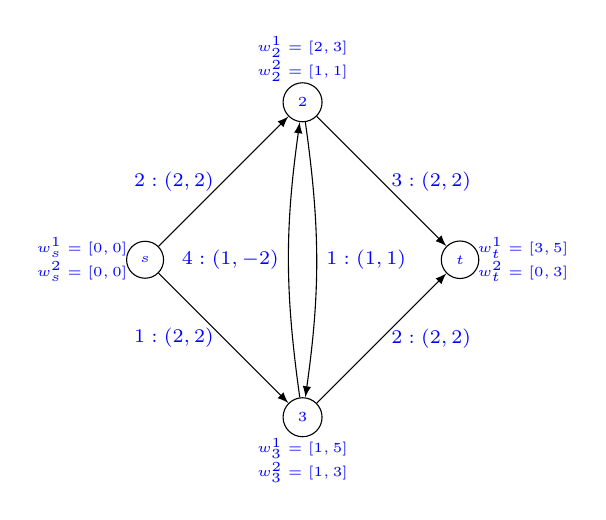
\begin{tikzpicture}[font=\tiny]
      %nodes
      \node at (-0.8, 0.15) {\blue{$w_s^1 = [0,0]$}};
      \node at (-0.8, -0.15) {\blue{$w_s^2 = [0,0]$}};
      \node[circle, draw] (s) at (0, 0) {\blue{$s$}};
      \node at (2, 2.7) {\blue{$w_2^1 = [2, 3]$}};
      \node at (2, 2.4) {\blue{$w_2^2 = [1, 1]$}};
      \node[circle, draw] (a) at (2, 2) {\blue{$2$}};
      \node at (2, -2.4) {\blue{$w_3^1 = [1, 5]$}};
      \node at (2, -2.7) {\blue{$w_3^2 = [1, 3]$}};
      \node[circle, draw] (b) at (2, -2) {\blue{$3$}};
      \node at (4.8, 0.15) {\blue{$w_t^1 = [3, 5]$}};
      \node at (4.8, -0.15) {\blue{$w_t^2 = [0, 3]$}};
      \node[circle, draw] (t) at (4, 0) {\blue{$t$}};
      %edges
      \path [draw,-latex] (s) to node[left]{\scriptsize\blue{$2: (2, 2)$}} (a);
      \path [draw,-latex] (s) to node[left]{\scriptsize\blue{$1: (2, 2)$}} (b);
      \path [draw,-latex] (a) to node[right]{\scriptsize\blue{$3: (2, 2)$}} (t);
      \path [draw,-latex] (b) to node[right]{\scriptsize\blue{$2: (2, 2)$}} (t);
      \path [draw,-latex] (a) edge [bend left=8] node[right]{\scriptsize\blue{$1: (1, 1)$}} (b);
      \path [draw,-latex] (b) edge [bend left=8] node[left]{\scriptsize\blue{$4: (1, -2)$}} (a);
    \end{tikzpicture}
    \caption{A ERCSPP instance digraph example.}
  \end{figure}
\end{frame}

\begin{frame}
  \frametitle{Problem definition}
  \blue{$c_a: (d^1_a, d^2_a)$}
  \begin{figure}[H]
    \centering
    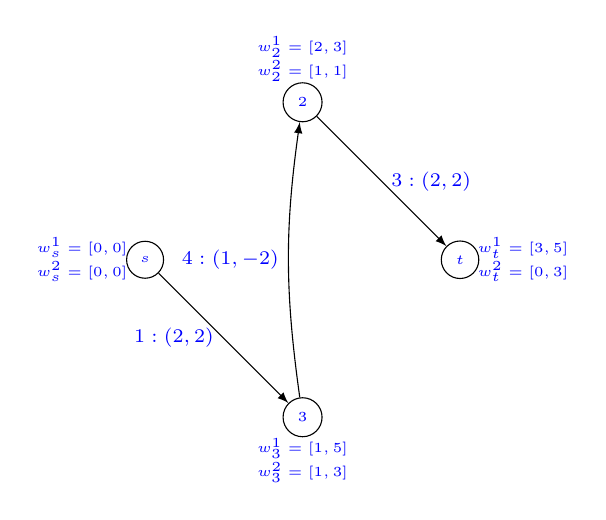
\begin{tikzpicture}[font=\tiny]
      %nodes
      \node at (-0.8, 0.15) {\blue{$w_s^1 = [0,0]$}};
      \node at (-0.8, -0.15) {\blue{$w_s^2 = [0,0]$}};
      \node[circle, draw] (s) at (0, 0) {\blue{$s$}};
      \node at (2, 2.7) {\blue{$w_2^1 = [2, 3]$}};
      \node at (2, 2.4) {\blue{$w_2^2 = [1, 1]$}};
      \node[circle, draw] (a) at (2, 2) {\blue{$2$}};
      \node at (2, -2.4) {\blue{$w_3^1 = [1, 5]$}};
      \node at (2, -2.7) {\blue{$w_3^2 = [1, 3]$}};
      \node[circle, draw] (b) at (2, -2) {\blue{$3$}};
      \node at (4.8, 0.15) {\blue{$w_t^1 = [3, 5]$}};
      \node at (4.8, -0.15) {\blue{$w_t^2 = [0, 3]$}};
      \node[circle, draw] (t) at (4, 0) {\blue{$t$}};
      %edges
      \path [draw,-latex] (s) to node[left]{\scriptsize\blue{$1: (2, 2)$}} (b);
      \path [draw,-latex] (b) edge [bend left=8] node[left]{\scriptsize\blue{$4: (1, -2)$}} (a);
      \path [draw,-latex] (a) to node[right]{\scriptsize\blue{$3: (2, 2)$}} (t);
    \end{tikzpicture}
    \caption{The solution of the previous instance.}
  \end{figure}
\end{frame}


\begin{frame}
  \begin{center}
    \Huge Mono-directional algorithm \footfullcite{FeilletDejaxGendreauGueguen2004}
  \end{center}
\end{frame}

\begin{frame}
  \begin{center}
    \Huge Properties
  \end{center}
\end{frame}

\begin{frame}
  \frametitle{Properties}
  \framesubtitle{Node state/label I}
  Let
  \begin{itemize}
    \item \blue{$i \in V$} be a node in \blue{$D$};
    \item \blue{$P_i$} be an elementary resource constrained \blue{$s$}-\blue{$i$}-path in \blue{$D$}; and 
    \item \blue{$S_i = (L_i = (l^1_i, ..., l^{|R|}_i), C_i)$} be the state or label of node \blue{$i$} in \blue{$P_i$}, where:
    \begin{itemize}
      \item \blue{$l^r_i \in \mathbb{R}$} is the amount of resource \blue{$r \in R$} consumed by \blue{$P_i$}; and 
      \item \blue{$C_i \in \mathbb{R}$} is the cost of path \blue{$P_i$}.
    \end{itemize}
  \end{itemize}
\end{frame}

\begin{frame}
  \frametitle{Properties}
  \framesubtitle{Node state/label I}
  \begin{figure}[H]
    \centering
    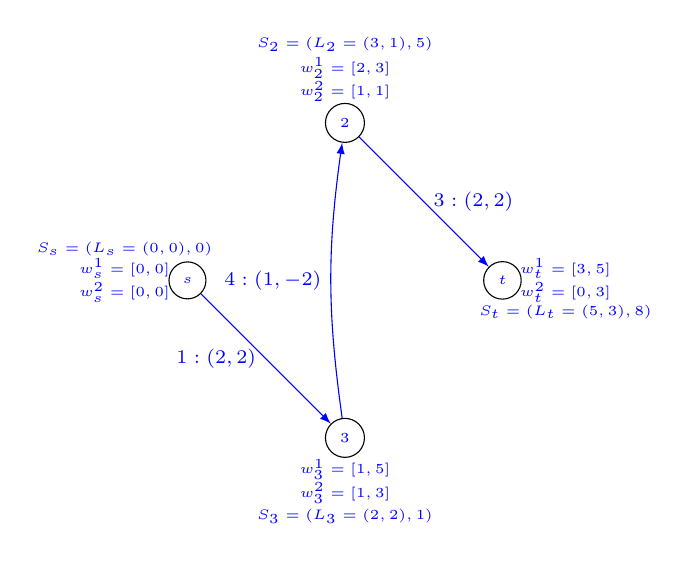
\begin{tikzpicture}[font=\tiny]
      %nodes
      \node at (-0.8, 0.4) {\blue{$S_s = (L_s = (0, 0), 0)$}};
      \node at (-0.8, 0.15) {\blue{$w_s^1 = [0,0]$}};
      \node at (-0.8, -0.15) {\blue{$w_s^2 = [0,0]$}};
      \node[circle, draw] (s) at (0, 0) {\blue{$s$}};
      \node at (2, 3) {\blue{$S_2 = (L_2 = (3, 1), 5)$}};
      \node at (2, 2.7) {\blue{$w_2^1 = [2, 3]$}};
      \node at (2, 2.4) {\blue{$w_2^2 = [1, 1]$}};
      \node[circle, draw] (a) at (2, 2) {\blue{$2$}};
      \node at (2, -2.4) {\blue{$w_3^1 = [1, 5]$}};
      \node at (2, -2.7) {\blue{$w_3^2 = [1, 3]$}};
      \node at (2, -3) {\blue{$S_3 = (L_3 = (2, 2), 1)$}};
      \node[circle, draw] (b) at (2, -2) {\blue{$3$}};
      \node at (4.8, 0.15) {\blue{$w_t^1 = [3, 5]$}};
      \node at (4.8, -0.15) {\blue{$w_t^2 = [0, 3]$}};
      \node at (4.8, -0.4) {\blue{$S_t = (L_t = (5, 3), 8)$}};
      \node[circle, draw] (t) at (4, 0) {\blue{$t$}};
      %edges
      \path [blue, draw,-latex] (s) to node[left]{\scriptsize\blue{$1: (2, 2)$}} (b);
      \path [blue, draw,-latex] (b) edge [bend left=8] node[left]{\scriptsize\blue{$4: (1, -2)$}} (a);
      \path [blue, draw,-latex] (a) to node[right]{\scriptsize\blue{$3: (2, 2)$}} (t);
    \end{tikzpicture}
    \caption{\blue{$P_s$}, \blue{$P_3$}, \blue{$P_2$}, and \blue{$P_t$}.}
  \end{figure}
\end{frame}

\begin{frame}
  \frametitle{Properties}
  \framesubtitle{Dominance I}
  Let
  \begin{itemize}
    \item \blue{$P_i$} and \blue{$P^{'}_i$} be two distinct elementary resource constrained \blue{$s$}-\blue{$i$}-paths in \blue{$D$}; and
    \item \blue{$S_i$} and \blue{$S^{'}_i$} be their respective labels.
  \end{itemize}
  \begin{definition}
    \blue{$P_i$} dominates \blue{$P^{'}_i \leftrightarrow S_i \leqslant S^{'}_i$}.
  \end{definition}
\end{frame}

\begin{frame}
  \frametitle{Properties}
  \framesubtitle{Node state/label II}
  Let
  \begin{itemize}
    \item \blue{$L_i = (l^1_i, ..., l^{|R|}_i, s_i, v_i^1, ..., v_i^{|V|})$} be the the  new resources state/label, where:
    \begin{itemize}
      \item \blue{$s_i = \sum_{j = 1}^{|V|} v_i^j = |V(P_i)|$} is the number of nodes visited by \blue{$P_i$}; and 
      \item \blue{$v_i^j \in \mathbb{B}$} is equals to \blue{$1$} if node \blue{$j \in V(P_i)$}, i.e., \blue{$j$} is visited by \blue{$P_i$}, such that \blue{$j \in V$}, and \blue{$0$} otherwise.
    \end{itemize}
  \end{itemize}
\end{frame}

\begin{frame}
  \frametitle{Properties}
  \framesubtitle{Node state/label II}
  \begin{figure}[H]
    \centering
    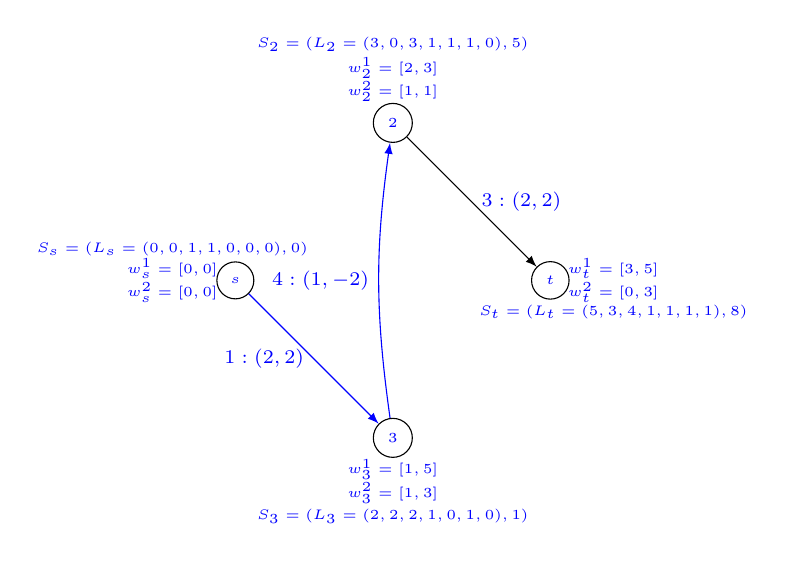
\begin{tikzpicture}[font=\tiny]
      %nodes
      \node at (-0.8, 0.4) {\blue{$S_s = (L_s = (0, 0, 1, 1, 0, 0, 0), 0)$}};
      \node at (-0.8, 0.15) {\blue{$w_s^1 = [0,0]$}};
      \node at (-0.8, -0.15) {\blue{$w_s^2 = [0,0]$}};
      \node[circle, draw] (s) at (0, 0) {\blue{$s$}};
      \node at (2, 3) {\blue{$S_2 = (L_2 = (3, 0, 3, 1, 1, 1, 0), 5)$}};
      \node at (2, 2.7) {\blue{$w_2^1 = [2, 3]$}};
      \node at (2, 2.4) {\blue{$w_2^2 = [1, 1]$}};
      \node[circle, draw] (a) at (2, 2) {\blue{$2$}};
      \node at (2, -2.4) {\blue{$w_3^1 = [1, 5]$}};
      \node at (2, -2.7) {\blue{$w_3^2 = [1, 3]$}};
      \node at (2, -3) {\blue{$S_3 = (L_3 = (2, 2, 2, 1, 0, 1, 0), 1)$}};
      \node[circle, draw] (b) at (2, -2) {\blue{$3$}};
      \node at (4.8, 0.15) {\blue{$w_t^1 = [3, 5]$}};
      \node at (4.8, -0.15) {\blue{$w_t^2 = [0, 3]$}};
      \node at (4.8, -0.4) {\blue{$S_t = (L_t = (5, 3, 4, 1, 1, 1, 1), 8)$}};
      \node[circle, draw] (t) at (4, 0) {\blue{$t$}};
      %edges
      \path [blue, draw,-latex] (s) to node[left]{\scriptsize\blue{$1: (2, 2)$}} (b);
      \path [blue, draw,-latex] (b) edge [bend left=8] node[left]{\scriptsize\blue{$4: (1, -2)$}} (a);
      \path [draw,-latex] (a) to node[right]{\scriptsize\blue{$3: (2, 2)$}} (t);
    \end{tikzpicture}
    \caption{\blue{$P_s$}, \blue{$P_3$}, \blue{$P_2$}, and \blue{$P_t$} with new labels.}
  \end{figure}
\end{frame}

\begin{frame}
  \frametitle{Properties}
  \framesubtitle{Dominance II}
  Let
  \begin{itemize}
    \item \blue{$P_i$} and \blue{$P^{'}_i$} be two distinct elementary paths from \blue{$s$} to \blue{$i \in V$} in \blue{$D$}; and
    \item \blue{$S_i$} and \blue{$S^{'}_i$} be the paths respective labels.
  \end{itemize}
  \begin{definition}
    \blue{$P_i$} dominates \blue{$P^{'}_i \leftrightarrow S_i \leqslant S^{'}_i$}.
  \end{definition}
  We can fastly check if \blue{$A = (v_i^1, ..., v_i^{|V|}) \leqslant B = (v_i^{1'}, ..., v_i^{|V|'})$} 
  by considering \blue{$A$} and \blue{$B$} as bitsets and checking whether 
  \blue{$(v_i^k \implies v_i^{k'}) \iff (\neg v_i^{k'} \vee v_i^k)$}, i.e. \blue{$(A \implies B) \iff (\neg B \vee A)$}, \blue{$\forall k \in \{1, ..., |V|\}$}.
  Hence, check whether a label dominates other can be done in \blue{$O(|R|)$}.
\end{frame}

\begin{frame}
  \frametitle{Properties}
  \framesubtitle{Unreachable nodes}
  \begin{definition}
  \blue{$k \in V$} is said to be unreachable by \blue{$P_i \rightarrow k \in V(P_i) \vee $} \blue{$ \exists r \in R (l_i^r + d_{ik}^r > e^r_k)$}.
  \end{definition}
  Note that, if \blue{$k \in V$} is unreachable by \blue{$P_i$}, then \blue{$\nexists$} elementary resource constrainted \blue{$i$}-\blue{$j$}-path in \blue{$D$}, due to the digraph metricity.
  That is the main reason why we are considering the digraph as complete and metric.
\end{frame}

\begin{frame}
  \frametitle{Properties}
  \framesubtitle{Node state/label III}
  Let
  \begin{itemize}
    \item \blue{$s_i = \sum_{j = 1}^{|V|} v_i^j$} be the number of unreachable nodes by the path \blue{$P_i$} at \blue{$i \in V(P_i)$}; and 
    \item \blue{$v_i^j \in \mathbb{B}$} be equals to \blue{$1$} if node \blue{$j \in V$} is unreachable by the path \blue{$P_i$}, and \blue{$0$} otherwise.
  \end{itemize}
\end{frame}

\begin{frame}
  \frametitle{Properties}
  \framesubtitle{Nondominated paths}
  \begin{claim}
    In order to find an ERCSPP optimal solution, suffices to consider only nondominated paths.
  \end{claim}
  \begin{claimproof}
    Let's consider two elementary resource constrained \blue{$s$}-\blue{$i$}-paths \blue{$P_i$} and \blue{$P^{'}_i$}, along with its labels \blue{$S_i$} and \blue{$S^{'}_i$}, such that \blue{$P_i$} dominates \blue{$P^{'}_i$}.
    Also, let's consider an arc \blue{$(i, j) \in \delta^{+}(i): \forall r \in R  $} \blue{$(l_i^{'r} + d_{ij}^r \leqslant e_j^r) \wedge v_i^{'j} = 0$}.
    Note that \blue{$\forall r \in R (l_i^r + d_{ij}^r \leqslant e_j^r) \wedge v_i^{j} = $} \blue{$0 \wedge C_i \leqslant C^{'}_i$}.
  \end{claimproof}
\end{frame}


\begin{frame}
  \begin{center}
    \Huge Algorithm
  \end{center}
\end{frame}

\begin{frame}
  \frametitle{Algorithm}
  \framesubtitle{Notations}
  Let
  \begin{itemize}
    \item \blue{$\Lambda_i$} be the list of labels on node \blue{$i \in V$};
    \item \blue{$N$} be the list of nodes to be processed;
    \item \blue{\[
        f(S_i) =  
        \begin{cases}
          \text{\textcolor{black}{true}},  & \text{\textcolor{black}{if} }      \forall r \in R (l_i^r \leqslant e_i^r) \wedge \forall j \in V (v_i^j \leqslant 1)\\
          \text{\textcolor{black}{false}}, & \text{\textcolor{black}{otherwise}}
        \end{cases}
    \]} be a function that says whether a label is feasible;
    \item \blue{$ E(S_i, j) = (l^r_i + d_{ij}^r : r \in R) \cup (s_i + 1, v_i^1, ..., v_i^j + 1, ..., v_i^{|V|}) $} be the function that returns the label resulting from the extension of a path \blue{$P_i$} from $s$ by a node \blue{$j$};
    \item \blue{$F_{ij}$} be the set of labels extended from \blue{$i \in V$} to \blue{$j \in V$}; and
    \item \blue{$N_D(\Lambda) = \{S_i \in \Lambda : \nexists S^{'}_i \in \Lambda (S^{'}_i \neq S_i \wedge S^{'}_i \leqslant S_i) \}$} be the function that returns all nondominated labels from \blue{$\Lambda$}.
  \end{itemize}
\end{frame}

\begin{frame}
  \frametitle{Algorithm}
  \framesubtitle{Code}
  \begin{algorithm}[H]
    \scriptsize
    \begin{algorithmic}[1]
      \REQUIRE \blue{$D(V, A), c_a \quad \forall a \in A, d_a^r \quad \forall a \in A, r \in R$}
      %initialization
      \STATE \blue{$\Lambda_s \gets \{ (\{0\}^{|R| + 1 + |V|}, 0) \}$};
      \STATE \blue{$\Lambda_i \gets \emptyset \quad \forall i \in V \backslash \{s\}$};
      \STATE \blue{$N \gets \{s\}$};
      %exploration
      \label{step:main_while}\WHILE {\blue{$N \neq \emptyset$}}
        \STATE Let \blue{$i \in N$} be a \blue{$N$} arbitrary node;
        \label{step:explore_arcs}\FORALL {\blue{$j \in \delta^{+}(i)$}}
          \STATE \blue{$F_{ij} \gets \emptyset$};
          \FORALL {\blue{$S_i \in \Lambda_i$}}
            \IF {\blue{$v_i^j = 0 \wedge f(E(S_i, j))$}}
              \STATE \blue{$F_{ij} \gets F_{ij} \cup \{E(S_i, j)\}$};
            \ENDIF
          \ENDFOR
          \STATE \blue{$\Lambda_j \gets N_D(F_{ij} \cup \Lambda_j)$};
          \IF {\blue{$\Lambda_j$} has changed}
            \STATE \blue{$N \gets N \cup \{j\}$};
          \ENDIF
        \ENDFOR
        \STATE \blue{$N \gets N \backslash \{i\}$};
      \ENDWHILE
    \end{algorithmic}
    \caption{Labeling algorithm}
    \label{alg:seq}
  \end{algorithm}
\end{frame}

\begin{frame}
  \frametitle{Algorithm}
  \framesubtitle{Example}
  \blue{$c_a: (d^1_a, d^2_a)$}\\
  \blue{$w_s^1 = w_s^2 = [0,0], w_2^1 = [2, 3], w_2^2 = [0, 1], w_3^1 = [1, 5], w_3^2 = [1, 3], w_t^1 = [3, 5], w_t^2 = [0, 2]$}
  \begin{multicols}{2}
    State before line \ref{step:main_while}:
    \begin{itemize}   
      \item \blue{$\Lambda_s = \{ ((0, 0, 1, 1, 0, 0, 0), 0) \}$};
      \item \blue{$\Lambda_2 = \Lambda_3 = \Lambda_t = \emptyset$};
      \item \blue{$N = \{\{s\}\}$};
    \end{itemize}   
    \begin{figure}[H]
      \centering
      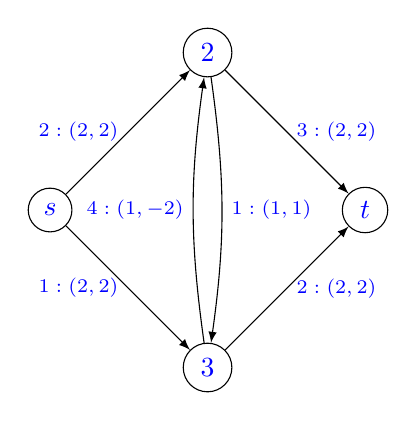
\begin{tikzpicture}
        %nodes
        \node[circle, draw] (s) at (0, 0) {\blue{$s$}};
        \node[circle, draw] (a) at (2, 2) {\blue{$2$}};
        \node[circle, draw] (b) at (2, -2) {\blue{$3$}};
        \node[circle, draw] (t) at (4, 0) {\blue{$t$}};
        %edges
        \path [draw,-latex] (s) to node[left]{\scriptsize\blue{$2: (2, 2)$}} (a);
        \path [draw,-latex] (s) to node[left]{\scriptsize\blue{$1: (2, 2)$}} (b);
        \path [draw,-latex] (a) to node[right]{\scriptsize\blue{$3: (2, 2)$}} (t);
        \path [draw,-latex] (b) to node[right]{\scriptsize\blue{$2: (2, 2)$}} (t);
        \path [draw,-latex] (a) edge [bend left=8] node[right]{\scriptsize\blue{$1: (1, 1)$}} (b);
        \path [draw,-latex] (b) edge [bend left=8] node[left]{\scriptsize\blue{$4: (1, -2)$}} (a);
      \end{tikzpicture}
      \caption{A ERCSPP instance digraph example.}
      \label{fig:vrptw_disposable_example}
    \end{figure}
  \end{multicols}
\end{frame}

\begin{frame}
  \frametitle{Algorithm}
  \framesubtitle{Example}
  \blue{$c_a: (d^1_a, d^2_a)$}\\
  \blue{$w_s^1 = w_s^2 = [0,0], w_2^1 = [2, 3], w_2^2 = [0, 1], w_3^1 = [1, 5], w_3^2 = [1, 3], w_t^1 = [3, 5], w_t^2 = [0, 2]$}
  \begin{multicols}{2}
    State at the end of \blue{$1$}st iteration of the while at line \ref{step:main_while}:
    \begin{itemize}   
      \item \blue{$\Lambda_s = \{ ((0, 0, 1, 1, 0, 0, 0), 0) \}$};
      \item \blue{$\Lambda_2 = \{((2, 2, 2, 1, 1, 0, 0), 2)\}$};
      \item \blue{$\Lambda_3 = \{((2, 2, 2, 1, 0, 1, 0), 1)\}$};
      \item \blue{$\Lambda_t = \emptyset$};
      \item \blue{$N = \{\{2\}, \{3\}\}$};
    \end{itemize}   
    \begin{figure}[H]
      \centering
      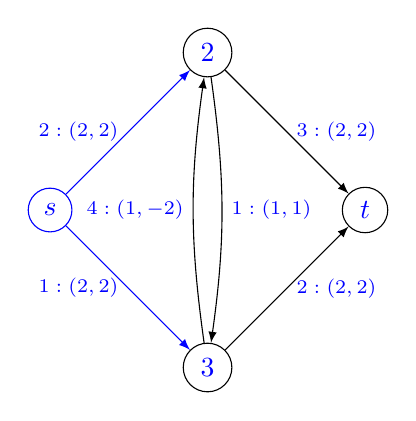
\begin{tikzpicture}
        %nodes
        \node[blue, circle, draw] (s) at (0, 0) {\blue{$s$}};
        \node[circle, draw] (a) at (2, 2) {\blue{$2$}};
        \node[circle, draw] (b) at (2, -2) {\blue{$3$}};
        \node[circle, draw] (t) at (4, 0) {\blue{$t$}};
        %edges
        \path [blue, draw,-latex] (s) to node[left]{\scriptsize\blue{$2: (2, 2)$}} (a);
        \path [blue, draw,-latex] (s) to node[left]{\scriptsize\blue{$1: (2, 2)$}} (b);
        \path [draw,-latex] (a) to node[right]{\scriptsize\blue{$3: (2, 2)$}} (t);
        \path [draw,-latex] (b) to node[right]{\scriptsize\blue{$2: (2, 2)$}} (t);
        \path [draw,-latex] (a) edge [bend left=8] node[right]{\scriptsize\blue{$1: (1, 1)$}} (b);
        \path [draw,-latex] (b) edge [bend left=8] node[left]{\scriptsize\blue{$4: (1, -2)$}} (a);
      \end{tikzpicture}
      \caption{Arcs explored the for loop at line \ref{step:explore_arcs} when \blue{$i = s$}.}
      \label{fig:vrptw_disposable_example}
    \end{figure}
  \end{multicols}
\end{frame}

\begin{frame}
  \frametitle{Algorithm}
  \framesubtitle{Example}
  \blue{$c_a: (d^1_a, d^2_a)$}\\
  \blue{$w_s^1 = w_s^2 = [0,0], w_2^1 = [2, 3], w_2^2 = [0, 1], w_3^1 = [1, 5], w_3^2 = [1, 3], w_t^1 = [3, 5], w_t^2 = [0, 2]$}
  \begin{multicols}{2}
    State at the end of \blue{$2$}nd iteration of the while at line \ref{step:main_while}:
    \begin{itemize}   
      \item \blue{$\Lambda_s = \{ ((0, 0, 1, 1, 0, 0, 0), 0) \}$};
    \item \blue{$\Lambda_2 = \{((2, 2, 2, 1, 1, 0, 0), 2)$} \blue{$, ((3, 0, 3, 1, 1, 1, 0), 5)\}$};
      \item \blue{$\Lambda_3 = \{((2, 2, 2, 1, 0, 1, 0), 1)\}$};
      \item \blue{$\Lambda_t = \emptyset$};
      \item \blue{$N = \{\{3\}, \{t\}, \{2\}\}$};
    \end{itemize}   
    \begin{figure}[H]
      \centering
      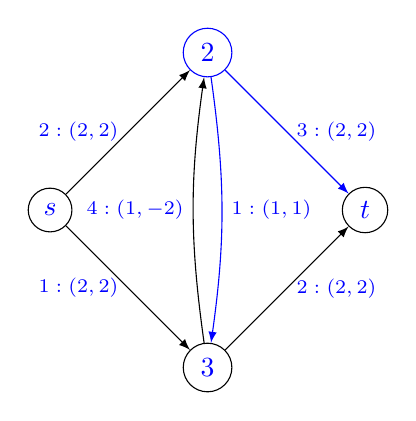
\begin{tikzpicture}
        %nodes
        \node[circle, draw] (s) at (0, 0) {\blue{$s$}};
        \node[blue, circle, draw] (a) at (2, 2) {\blue{$2$}};
        \node[circle, draw] (b) at (2, -2) {\blue{$3$}};
        \node[circle, draw] (t) at (4, 0) {\blue{$t$}};
        %edges
        \path [draw,-latex] (s) to node[left]{\scriptsize\blue{$2: (2, 2)$}} (a);
        \path [draw,-latex] (s) to node[left]{\scriptsize\blue{$1: (2, 2)$}} (b);
        \path [blue, draw,-latex] (a) to node[right]{\scriptsize\blue{$3: (2, 2)$}} (t);
        \path [draw,-latex] (b) to node[right]{\scriptsize\blue{$2: (2, 2)$}} (t);
        \path [blue, draw,-latex] (a) edge [bend left=8] node[right]{\scriptsize\blue{$1: (1, 1)$}} (b);
        \path [draw,-latex] (b) edge [bend left=8] node[left]{\scriptsize\blue{$4: (1, -2)$}} (a);
      \end{tikzpicture}
      \caption{Arcs explored the for loop at line \ref{step:explore_arcs} when \blue{$i = 2$}.}
      \label{fig:vrptw_disposable_example}
    \end{figure}
  \end{multicols}
\end{frame}

\begin{frame}
  \frametitle{Algorithm}
  \framesubtitle{Example}
  \blue{$c_a: (d^1_a, d^2_a)$}\\
  \blue{$w_s^1 = w_s^2 = [0,0], w_2^1 = [2, 3], w_2^2 = [0, 1], w_3^1 = [1, 5], w_3^2 = [1, 3], w_t^1 = [3, 5], w_t^2 = [0, 2]$}
  \begin{multicols}{2}
    State at the end of \blue{$3$}rd iteration of the while at line \ref{step:main_while}:
    \begin{itemize}   
      \item \blue{$\Lambda_s = \{ ((0, 0, 1, 1, 0, 0, 0), 0) \}$};
      \item \blue{$\Lambda_2 = \{((2, 2, 2, 1, 1, 0, 0), 2)$} \blue{$, ((3, 0, 3, 1, 1, 1, 0), 5)\}$};
      \item \blue{$\Lambda_3 = \{((2, 2, 2, 1, 0, 1, 0), 1)\}$};
      \item \blue{$\Lambda_t = \{((5, 2, 4, 1, 1, 1, 1), 8)\}$};
      \item \blue{$N = \{\{t\}, \{2\}\}$};
    \end{itemize}   
    \begin{figure}[H]
      \centering
      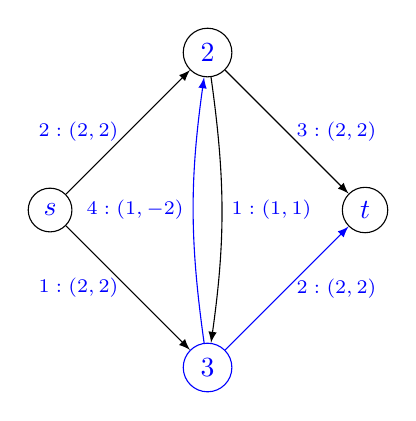
\begin{tikzpicture}
        %nodes
        \node[circle, draw] (s) at (0, 0) {\blue{$s$}};
        \node[circle, draw] (a) at (2, 2) {\blue{$2$}};
        \node[blue, circle, draw] (b) at (2, -2) {\blue{$3$}};
        \node[circle, draw] (t) at (4, 0) {\blue{$t$}};
        %edges
        \path [draw,-latex] (s) to node[left]{\scriptsize\blue{$2: (2, 2)$}} (a);
        \path [draw,-latex] (s) to node[left]{\scriptsize\blue{$1: (2, 2)$}} (b);
        \path [draw,-latex] (a) to node[right]{\scriptsize\blue{$3: (2, 2)$}} (t);
        \path [blue, draw,-latex] (b) to node[right]{\scriptsize\blue{$2: (2, 2)$}} (t);
        \path [draw,-latex] (a) edge [bend left=8] node[right]{\scriptsize\blue{$1: (1, 1)$}} (b);
        \path [blue, draw,-latex] (b) edge [bend left=8] node[left]{\scriptsize\blue{$4: (1, -2)$}} (a);
      \end{tikzpicture}
      \caption{Arcs explored the for loop at line \ref{step:explore_arcs} when \blue{$i = 3$}.}
      \label{fig:vrptw_disposable_example}
    \end{figure}
  \end{multicols}
\end{frame}

\begin{frame}
  \frametitle{Algorithm}
  \framesubtitle{Example}
  \blue{$c_a: (d^1_a, d^2_a)$}\\
  \blue{$w_s^1 = w_s^2 = [0,0], w_2^1 = [2, 3], w_2^2 = [0, 1], w_3^1 = [1, 5], w_3^2 = [1, 3], w_t^1 = [3, 5], w_t^2 = [0, 2]$}
  \begin{multicols}{2}
    State at the end of \blue{$4$}th iteration of the while at line \ref{step:main_while}:
    \begin{itemize}   
      \item \blue{$\Lambda_s = \{ ((0, 0, 1, 1, 0, 0, 0), 0) \}$};
      \item \blue{$\Lambda_2 = \{((2, 2, 2, 1, 1, 0, 0), 2)$} \blue{$, ((3, 0, 3, 1, 1, 1, 0), 5)\}$};
      \item \blue{$\Lambda_3 = \{((2, 2, 2, 1, 0, 1, 0), 1)\}$};
      \item \blue{$\Lambda_t = \{((5, 2, 4, 1, 1, 1, 1), 8)\}$};
      \item \blue{$N = \{\{2\}\}$};
    \end{itemize}   
    \begin{figure}[H]
      \centering
      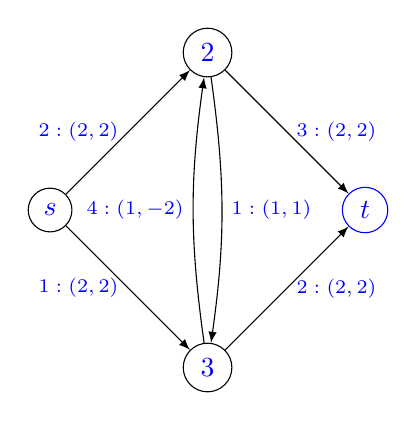
\begin{tikzpicture}
        %nodes
        \node[circle, draw] (s) at (0, 0) {\blue{$s$}};
        \node[circle, draw] (a) at (2, 2) {\blue{$2$}};
        \node[circle, draw] (b) at (2, -2) {\blue{$3$}};
        \node[blue, circle, draw] (t) at (4, 0) {\blue{$t$}};
        %edges
        \path [draw,-latex] (s) to node[left]{\scriptsize\blue{$2: (2, 2)$}} (a);
        \path [draw,-latex] (s) to node[left]{\scriptsize\blue{$1: (2, 2)$}} (b);
        \path [draw,-latex] (a) to node[right]{\scriptsize\blue{$3: (2, 2)$}} (t);
        \path [draw,-latex] (b) to node[right]{\scriptsize\blue{$2: (2, 2)$}} (t);
        \path [draw,-latex] (a) edge [bend left=8] node[right]{\scriptsize\blue{$1: (1, 1)$}} (b);
        \path [draw,-latex] (b) edge [bend left=8] node[left]{\scriptsize\blue{$4: (1, -2)$}} (a);
      \end{tikzpicture}
      \caption{Arcs explored the for loop at line \ref{step:explore_arcs} when \blue{$i = t$}.}
      \label{fig:vrptw_disposable_example}
    \end{figure}
  \end{multicols}
\end{frame}

\begin{frame}
  \frametitle{Algorithm}
  \framesubtitle{Example}
  \blue{$c_a: (d^1_a, d^2_a)$}\\
  \blue{$w_s^1 = w_s^2 = [0,0], w_2^1 = [2, 3], w_2^2 = [0, 1], w_3^1 = [1, 5], w_3^2 = [1, 3], w_t^1 = [3, 5], w_t^2 = [0, 2]$}
  \begin{multicols}{2}
    State at the end of \blue{$5$}th iteration of the while at line \ref{step:main_while}:
    \begin{itemize}   
      \item \blue{$\Lambda_s = \{ ((0, 0, 1, 1, 0, 0, 0), 0) \}$};
      \item \blue{$\Lambda_2 = \{((2, 2, 2, 1, 1, 0, 0), 2)$} \blue{$, ((3, 0, 3, 1, 1, 1, 0), 5)\}$};
      \item \blue{$\Lambda_3 = \{((2, 2, 2, 1, 0, 1, 0), 1)\}$};
      \item \blue{$\Lambda_t = \{((5, 2, 4, 1, 1, 1, 1), 8)\}$};
      \item \blue{$N = \{\}$};
    \end{itemize}   
    \begin{figure}[H]
      \centering
      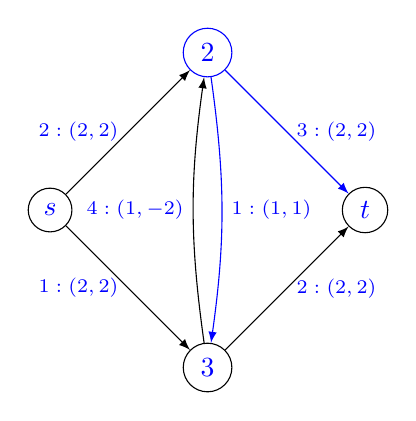
\begin{tikzpicture}
        %nodes
        \node[circle, draw] (s) at (0, 0) {\blue{$s$}};
        \node[blue, circle, draw] (a) at (2, 2) {\blue{$2$}};
        \node[circle, draw] (b) at (2, -2) {\blue{$3$}};
        \node[circle, draw] (t) at (4, 0) {\blue{$t$}};
        %edges
        \path [draw,-latex] (s) to node[left]{\scriptsize\blue{$2: (2, 2)$}} (a);
        \path [draw,-latex] (s) to node[left]{\scriptsize\blue{$1: (2, 2)$}} (b);
        \path [blue, draw,-latex] (a) to node[right]{\scriptsize\blue{$3: (2, 2)$}} (t);
        \path [draw,-latex] (b) to node[right]{\scriptsize\blue{$2: (2, 2)$}} (t);
        \path [blue, draw,-latex] (a) edge [bend left=8] node[right]{\scriptsize\blue{$1: (1, 1)$}} (b);
        \path [draw,-latex] (b) edge [bend left=8] node[left]{\scriptsize\blue{$4: (1, -2)$}} (a);
      \end{tikzpicture}
      \caption{Arcs explored the for loop at line \ref{step:explore_arcs} when \blue{$i = 2$}.}
      \label{fig:vrptw_disposable_example}
    \end{figure}
  \end{multicols}
\end{frame}


\begin{frame}
  \begin{center}
    \Huge Bi-directional algorithm \footfullcite{RighiniSalani2006}
  \end{center}
\end{frame}

\begin{frame}
  \frametitle{Bi-directional search}
  \framesubtitle{Previous algorithm analysis}
  \begin{itemize}
    \item The number of generated states increases rapidly according to the size of the instance;
    \item Among the reasons it is that any node \blue{$i$} label extension generates as many other labels as the number of \blue{$i$} possible successors;
    \item States are pruned only when they are dominated;
  \end{itemize}
\end{frame}

\begin{frame}
  \frametitle{Bi-directional search}
  \framesubtitle{Improvements}
  Consider labels being propagated both from \blue{$s$} to \blue{$t$} and vice-versa.
  Let
  \begin{itemize}
    \item \blue{$P^{'}_j$} be a feasible \blue{$j$}-\blue{$t$}-path in \blue{$D$};
    \item \blue{$\Lambda_i^{f}$} and \blue{$\Lambda_i^{b}$} be the sets of forward and backward labels of node \blue{$i \in V$};
    \item \blue{$E^b(S_j, i) = (\text{max} \{l^r_j - d_{ij}^r, (\textcolor{black}{max}_{i^{'} \in V} e^r_i) - b^r_i\} : r \in R) \cup (s_i + 1, v_i^1, ..., v_i^j + 1, $} \blue{$..., v_i^{|V|}) $} be the function that returns the label resulting from the backwards extension of a path \blue{$P^{'}_j$} by a node \blue{$i$} (\blue{$O(|R|)$}).
    \item \blue{\[
        f^b(S_j, i) =  
        \begin{cases}
          \text{\textcolor{black}{true}},  & \text{\textcolor{black}{if} }      \forall r \in R (l^r_j - d_{ij}^r \leqslant e_i^r) \wedge \neg v_j^i\\
          \text{\textcolor{black}{false}}, & \text{\textcolor{black}{otherwise}}
        \end{cases}
    \]} be a function that says whether a backward extension is feasible (\blue{$O(|R|)$});
 %the algorithm must examine two subsets of states, 
 %whose size grows exponentially with the number of arcs in the corresponding forward and backward paths. 
 %Due to the exponential dependence on the number of steps, 
 %it is intuitive that generating shorter paths may yield a significant advantage in terms of number of states considered, 
 %provided that duplicate solutions are avoided. 
 %This is precisely the effect of bounding, whose purpose is to limit the length of the paths corresponding to non-dominated states. 
 %Hereafter we formally define our bounded bi-directional dynamic programming algorithm.
    %States, recurrence equations and domination rules are symmetrical to those presented above.
  \end{itemize}
\end{frame}

\begin{frame}
  \frametitle{Bi-directional search}
  \framesubtitle{Improvements}
  Let
  \begin{itemize}
    \item \blue{$i, j \in V : i \neq j$} be two distinct nodes;
    \item \blue{$S_i = (L_i, C_i) \in \Lambda_i^{f}$} be a forward state of node \blue{$i$}; and 
    \item \blue{$S_j = (L_j, C_j) \in \Lambda_j^{b}$} be a backward state of node \blue{$j$}.
  \end{itemize}
  \begin{definition}
    Forward state \blue{$S_i$} and a backward state \blue{$S_j$} can be feasibly joined through arc \blue{$(i, j)$} 
    if \blue{$(\neg ((v_i^1, ..., v_i^{|V|}) \vee (v_j^1, ..., v_j^{|V|}))$}, and \blue{$ l_j^r - d_{ij}^r \geqslant l_i^r  $}.
  \end{definition}
  A path from \blue{$s$} to \blue{$t$} is detected each time a forward state in \blue{$\Lambda_i^{f}$} and a backward state in \blue{$\Lambda_j^{b}$} can be feasibly joined through arc \blue{$(i, j)$}.
%If there exist a resource whose consumption is not less than a certain known amount β at each extension, then it is possible to define buckets of size β and to mark as permanent all those labels for which the resource consumption falls in the range of the first bucket not yet extended. 
\end{frame}

\begin{frame}
  \frametitle{Bi-directional search}
  \framesubtitle{Algorithm: Forward extension procedure}
  \begin{algorithm}[H]
    \scriptsize
    \begin{algorithmic}[1]
      \STATE Function\{Forward extension\}\{\blue{$i \in V, \Lambda^f_i, N$}\}
        \label{algo2:setp:explore_arcs}\FORALL {\blue{$(i, j) \in \delta^{+}(i)$}}
          \STATE \blue{$F_{ij} \gets \emptyset$};
          \FORALL {\blue{$S_i \in \Lambda^f_i$}}
            \IF {\blue{$f(S_i, j)$}}
              \STATE \blue{$F_{ij} \gets F_{ij} \cup \{E(S_i, j)\}$};
            \ENDIF
          \ENDFOR
          \STATE \blue{$\Lambda^f_j \gets N_D(F_{ij} \cup \Lambda^f_j)$};
          \IF {\blue{$\Lambda^f_j$} has changed}
            \STATE \blue{$N \gets N \cup \{j\}$};
          \ENDIF
        \ENDFOR
        \STATE \blue{$N \gets N \backslash \{i\}$};
     \STATE EndFunction
    \end{algorithmic}
    \caption{Forward extension algorithm}
    \label{alg2:forward_extension}
  \end{algorithm}
\end{frame}

\begin{frame}
  \frametitle{Bi-directional search}
  \framesubtitle{Algorithm: Backward extension procedure}
  \begin{algorithm}[H]
    \scriptsize
    \begin{algorithmic}[1]
      \STATE Function\{Backward extension\}\{\blue{$i \in V, \Lambda^b_i, N$}\}
        \label{algo3:setp:explore_arcs}\FORALL {\blue{$(j, i) \in \delta^{-}(i)$}}
          \STATE \blue{$F_{ji} \gets \emptyset$};
          \FORALL {\blue{$S_i \in \Lambda^b_i$}}
            \IF {\blue{$f^b(S_i, j)$}}
              \STATE \blue{$F_{ji} \gets F_{ji} \cup \{E^b(S_i, j)\}$};
            \ENDIF
          \ENDFOR
          \STATE \blue{$\Lambda^b_j \gets N_D(F_{ji} \cup \Lambda^b_j)$};
          \IF {\blue{$\Lambda^b_j$} has changed}
            \STATE \blue{$N \gets N \cup \{j\}$};
          \ENDIF
        \ENDFOR
        \STATE \blue{$N \gets N \backslash \{i\}$};
     \STATE EndFunction
    \end{algorithmic}
    \caption{Forward extension algorithm}
    \label{alg3:backward_extension}
  \end{algorithm}
\end{frame}


\begin{frame}
  \frametitle{Bi-directional search}
  \framesubtitle{Algorithm: Search}
  \begin{algorithm}[H]
    \scriptsize
    \begin{algorithmic}[1]
      \REQUIRE \blue{$D(V, A), c_a \quad \forall a \in A, d_a^r \quad \forall a \in A, r \in R$}
      %initialization
      \STATE \blue{$\Lambda^f_s \gets \{ (\{0\}^{|R|} \cup (1, 1) \cup \{0\}^{|V| - 1}, 0) \}$};
      \STATE \blue{$\Lambda^b_t \gets \{ (e_t^r : r \in R) \cup (1, 1) \cup \{0\}^{|V| - 1}, 0) \}$};
      \STATE \blue{$\Lambda^f_i \gets \emptyset \quad \forall i \in V \backslash \{s\}$};
      \STATE \blue{$\Lambda^b_i \gets \emptyset \quad \forall i \in V \backslash \{t\}$};
      \STATE \blue{$N \gets \{s, t\}$};
      %exploration
      \label{algo1:setp:main_while}\WHILE {\blue{$N \neq \emptyset$}}
        \STATE Let \blue{$i \in N$} be a \blue{$N$} arbitrary node;
        \STATE Forward extension\{\blue{$i, \Lambda^f_i, N$}\};
        \STATE Backward extension\{\blue{$i, \Lambda^b_i, N$}\};
        \STATE \blue{$N \gets N \backslash \{i\}$};
      \ENDWHILE
      \STATE \{Merge\}\{\blue{$ \Lambda^f, \Lambda^b, N$}\};
     % \RETURN \blue{min$_{(L_t, C_t) \in \Lambda_t} \{ C_t \}$} if \blue{$\Lambda_t \neq \emptyset$} else \blue{$\infty$};
    \end{algorithmic}
    \caption{Search}
    \label{alg3:main}
  \end{algorithm}
\end{frame}

\begin{frame}
  \frametitle{Bi-directional search}
  \framesubtitle{Strategies}
  \begin{itemize}
    \item Bounding for pruning;
    \item Halfway bounding for the number of extensions;
    \item Bounding for monotone resources;
    \item Solutions uniqueness.
  \end{itemize}
\end{frame}

\begin{frame}
  \frametitle{Bi-directional search}
  \framesubtitle{Bounding for pruning}
  Let
  \begin{itemize}
    \item \blue{$S_i = (L_i, C_i) \in \Lambda^f_i$} be a forward state of node \blue{$i \in V$};
    \item \blue{$\mathcal{S} = \{j \in V : v_i^j\} = V(P_i)$} be the set of nodes in \blue{$P_i$};
    \item \blue{$m^f_r(S_i, j) = \textcolor{black}{min}_{k \notin \mathcal{S} \backslash \{i\}} \{ d^r_{kj} \}$} be a lower bound to the consumption of resource \blue{$r \in R$} when a forward state \blue{$S_i$} is extended to \blue{$j \in V$};
    \item \blue{$S^{'}_i = (L^{'}_i, C^{'}_j) \in \Lambda^b_i$} be a forward state of node \blue{$i \in V$};
    \item \blue{$m^b_r(S_i, j) = \textcolor{black}{min}_{k \notin \mathcal{S} \backslash \{i\}} \{ d^r_{jk} \}$} be a lower bound to the consumption of resource \blue{$r \in R$} when the backward state \blue{$S^{'}_i$} is extended to \blue{$j \in V$};
  \end{itemize}
\end{frame}

\begin{frame}
  \frametitle{Bi-directional search}
  \framesubtitle{Bounding for pruning}
 \begin{align} 
    \textcolor{black}{min}  && \color{blue}\sum_{j \in V \backslash \mathcal{S}} \lambda_j \textcolor{black}{min}_{k \notin \mathcal{S}\backslash \{i\}} \{ c_{kj} \} && \\
    \textcolor{black}{s.t.} && \color{blue}l_i^r + \sum_{j \in V \backslash \mathcal{S}} \lambda_j m^f_r(S_i, j) \leqslant e_r^i && \color{blue}\forall r \in R \\
                            && \color{blue}\lambda_j \in \mathbb{B} && \color{blue}\forall j \in V \backslash \mathcal{S} 
\end{align}
  Let \blue{$\bar{C}_i$} be the optimal solution of the above knapsack formulation for the label \blue{$S_i$}, and \blue{$UB$} be an upper bound on the ERCSPP solution.
  If \blue{$C_i - \bar{C}_i \geqslant UB$} then the state \blue{$S_i$} can be chopped off.
\end{frame}

\begin{frame}
  \frametitle{Bi-directional search}
  \framesubtitle{Halfway bounding for the number of extensions}
  \begin{align} 
    \textcolor{black}{min}  && \color{blue}\sum_{j \in V \backslash \mathcal{S}} \lambda_j && \\
    \textcolor{black}{s.t.} && \color{blue}l_i^r + \sum_{j \in V \backslash \mathcal{S}} \lambda_j m^f_r(S_i, j) \leqslant e_r^i && \color{blue}\forall r \in R \\
                            && \color{blue}\lambda_j \in \mathbb{B} && \color{blue}\forall j \in V \backslash \mathcal{S} 
  \end{align}
  If the optimal solution \blue{$p$} of the above knapsack formulation is \blue{$\leqslant |\mathcal{S}|$} then the state \blue{$S_i$} has reached its halfway, since we are working with bi-directional search, then we can stop the extensions of this state.
\end{frame}

\begin{frame}
  \frametitle{Bi-directional search}
  \framesubtitle{Bounding for monotone resources}
  Let \blue{$r \in R$} be a resource, \blue{$r$} is said to be monotone iff \blue{$d_a^r \geqslant 0$} \blue{$\forall a \in A$}.
  If \blue{$l_i^r \geqslant \frac{e^r_t}{2}$} then the state \blue{$S_i$} has reached its resource halfway, then we can stop the extensions of this state.
\end{frame}

\begin{frame}
  \frametitle{Bi-directional search}
  \framesubtitle{Solutions uniqueness}
  \begin{itemize}
    \item Another issue to be considered comes from the need of generating many different columns with negative reduced cost when using the ERCSPP as a pricing subproblem in a branch-and-price;
    \item The bounded bi-directional dynamic programming algorithm can provide duplicate solutions: 
      \begin{itemize}
        \item Consider for instance an \blue{$s$}-\blue{$t$} path including the sequence \blue{$(i, j, k)$};
        \item Eventually, the forward states for vertices \blue{$i$} and \blue{$j$} and backward states for vertices \blue{$j$} and \blue{$k$} are generated;
        \item Hence the same solution is obtainable by merging a forward state of \blue{$i$} with a backward state of \blue{$j$},
          or merging a forward state of \blue{$j$} with a backward state of \blue{$k$};
        \item If we need to store in some data structure all columns with negative reduced cost, the duplicate columns cannot be discarded on the basis of their cost and their identification may be computationally expensive.
      \end{itemize}
  \end{itemize}
\end{frame}

\begin{frame}
  \frametitle{Bi-directional search}
  \framesubtitle{Solutions uniqueness}
  \begin{itemize}
    \item Then, we accept an \blue{$s$}-\blue{$t$} path only when it is produced by the join of a forward state and a backward state,
      which the forward and backward consumptions of a monotone resource are as close as possible to half the overall consumption (\blue{$\frac{e^r_t}{2}$}),
      that is the two states are as close as possible to the halfway point along the \blue{$s$}-\blue{$t$} path;
    \item Let $\rho_f$ and $\rho_b$ be a monotone resource consumption in forward and backward paths;
    \item Among all possible pairs of forward and backward states producing the same \blue{$s$}-\blue{$t$} path we choose the one which \blue{$\psi = |\rho_f - \rho_b|$} is minimum;
    \item In the case of a tie, i.e., two available mergings where \blue{$\psi$} is minimum, we choose the one with \blue{$\rho_f > \rho_b$};
    \item This test guarantees that each \blue{$s$}–\blue{$t$} path is generated only once.
  \end{itemize}
\end{frame}

\begin{frame}
  \frametitle{Bi-directional search}
  \framesubtitle{Algorithm: Merge}
  Let
  \begin{itemize}
    \item \blue{\[
        f(S_i, S_j) =  
        \begin{cases}
        \text{\textcolor{black}{true}},  & \text{\textcolor{black}{if} } \forall r \in R (l^r_j - d_{ij}^r \leqslant e_i^r) \wedge \\
                                         & (v_i^1, ..., v_i^{|V|}) \implies \neg (v_j^1, ..., v_j^{|V|})\\
          \text{\textcolor{black}{false}}, & \text{\textcolor{black}{otherwise}}
        \end{cases}
    \]} be a function that says whether a merge between a forward label \blue{$S_i$} and a backward label \blue{$S_j$} is feasible;
    \item \blue{$H(S_i, S_j)$} be the function that checks if the \blue{$s$}-\blue{$t$} path obtained from merging the forward label \blue{$S_i$} and the backward label \blue{$S_j$} satisfies the halfway conditions outlined before (Bounding for monotone resources, and Halfway bounding for the number of extensions);
    \item \blue{$Save(S_i, S_j)$} a function tha saves the solution obtained from the two merging of \blue{$S_i$} and \blue{$S_j$}.
  \end{itemize}
\end{frame}

\begin{frame}
  \frametitle{Bi-directional search}
  \framesubtitle{Algorithm: Merge}
  \begin{algorithm}[H]
    \scriptsize
    \begin{algorithmic}[1]
     \STATE Function\{Merge forward and backward paths\}\{\blue{$ i, \Lambda^f_i, \Lambda^b_i $}\}
       \STATE Let \blue{$\phi_i^f = \textcolor{black}{min}_{(L_i, C_i) \in \Lambda^f_i} \{ C_i \}$} be the minimum cost among all labels in \blue{$\Lambda^f_i$};
       \STATE Let \blue{$\phi_i^b = \textcolor{black}{min}_{(L_i, C_i) \in \Lambda^b_i} \{ C_i \}$} be the minimum cost among all labels in \blue{$\Lambda^b_i$};
       \STATE Let \blue{$\phi^b = \textcolor{black}{min}_{i \in V} \{ \phi_i^b \}$} be the minimum cost among all labels in \blue{$\Lambda^b$};
       \FORALL {\blue{$i \in V$}}
         \IF {\blue{$\phi_i^f + \textcolor{black}{min}_{j \in V \backslash \{i\}} c_{ij} + \phi^b < UB$}}
           \FORALL {\blue{$S_i = (L_i, C_i) \in \Lambda_i^f$}}
             \IF {\blue{$C_i + \textcolor{black}{min}_{j \in V \backslash \{i\}} c_{ij} + \phi^b < UB$}}
               \FORALL {\blue{$j \in V$}}
                 \IF {\blue{$C_i + c_{ij} + \phi_j^b < UB$}}
                   \FORALL {\blue{$S_j = (L_j, C_j) \in \Lambda_j^b$}}
                     \IF {\blue{$C_i + c_{ij} + C_j < UB \wedge f(S_i, S_j) \wedge H(S_i, S_j)$}}
                       \STATE \blue{$Save(S_i, S_j)$};
                     \ENDIF
                   \ENDFOR
                 \ENDIF
               \ENDFOR
             \ENDIF
           \ENDFOR
         \ENDIF
       \ENDFOR
     \STATE EndFunction
    \end{algorithmic}
    \caption{Merge forward and backward paths algorithm}
    \label{alg3:backward_extension}
  \end{algorithm}
\end{frame}


\begin{frame}
\printbibliography
\end{frame}

\end{document}
